\documentclass[a4paper]{article}
\usepackage[english]{babel}
\usepackage[utf8]{inputenc}
\usepackage{amsmath}
\usepackage{graphicx}
\usepackage{caption}
\usepackage{url}
\usepackage{lscape}
\usepackage{placeins}
\usepackage[official]{eurosym}
\usepackage{setspace}
\usepackage{hyperref}
\usepackage{booktabs, multirow} % for borders and merged ranges
\usepackage[table]{xcolor} % for cell colors
\usepackage[left=3cm, right=3cm, top = 1.5cm, bottom=1.5cm]{geometry}
\onehalfspacing
\renewcommand{\thesection}{\Alph{section}}


\title{TD Gestion de projet}
\author{Hexanome 4121}

\date{27 Septembre 2021}

\usepackage[T1]{fontenc}
\begin{document}
\maketitle

\begin{figure}[h]
\centering

\includegraphics[width=0.4\textwidth]{Logo_INSA.png}
\end{figure}

\begin{center}
Dossier de gestion de projet de l'hexanome 4121 composé de S.VOLTZ, A.STRAPPAZZON, R.GALLÉ, F.VILLEGAS, A.BEN SALEM, F.RASCOUSSIER et T.PIRES
\end{center}

\newpage

\tableofcontents

	
	\newpage
	\section{Objet du projet - Contexte}
Dans le cadre de sa transformation digitale, le groupe pétrolier Petrolif souhaite disposer d’un tissu applicatif complet permettant le suivi en temps réel de ses infrastructures. Cette surveillance continue doit permettre de signaler rapidement toute anomalie sur l’ensemble de ses opérations et assurer un service d’assistance grâce à une application d’aide à la décision. L’objectif principal est de faciliter le travail des responsables pour leur permettre d’effectuer les choix adéquats. Les objectifs principaux sont d’assurer le suivi des interventions effectuées; de faciliter l’accès à un ensemble de services; de lister et de localiser les opérations de maintenance à réaliser; et de permettre d'effectuer des opérations de configuration et de maintenance à distance des dispositifs matériels.

Ce présent document d’initialisation couvre le sous-projet relatif au lot « Application » dont le périmètre s'étend au développement complet de 4 applications utilisateurs. Les applications ont pour objectif respectivement la configuration des capteurs, la surveillance des sites grâce aux capteurs, la gestion et la maintenance des données. Le développement se fera selon la méthode SCRUM. 

Ce document présente la conception générale, les spécifications, la gestion du projet ainsi que l’évaluation des risques ou encore le contrôle qualité relatif au développement des applications traitées.
	\newpage
	
	
	
	
	
	
	\section{Résultats (livrables) attendus - PBS}
                
	    \subsection{Dossier de production}
	        \begin{itemize}
	        \item Documentation \begin{itemize}
	                \item Documentation technique
	                \item Documentation utilisateur
	            \end{itemize}
	        \item Spécifications techniques et fonctionnelles
	            \begin{itemize}
	                \item Contexte/Objectifs/Périmètre du projet
	                \item Modélisation
	                \item Architecture applicative
	                \item Diagrammes UML de l'application
	                \begin{itemize}
	                    \item Diagramme de classe
	                    \item Diagramme de séquence
	                    \item Diagramme d'état
	                    \item Diagramme d'activité
	                \end{itemize}
	                \item Dossier de spécifiaction fonctionnelles (SFG + SFD)
	                \item Dossier de spécification non-fonctionnelles
	                \item Dossier de spécification technique
	                \item Évaluation des coûts, mise en place du budget
	                \item Maquettes de l'application
	        \end{itemize}
	        \item Logiciel (cf. \hyperlink{logiciel}{\S B.3} )
	            \begin{itemize}
	                \item Application A1: Configuration des capteurs
	                \item Application A2: Surveillance
	                \item Application A3: Gestion
	                \item Application A4: MAintenance
	            \end{itemize}
	        \end{itemize}
	    \subsection{Dossier de gestion projet}
	    \begin{itemize}
	        \item Dossier d'initialisation
                \begin{itemize}
                    \item PBS
                    \item WBS
                        \begin{itemize}
                            \item Diagramme de Gantt
                            
                        \end{itemize}
                    \item OBS
                    \item Évaluation des risques de sécurité
                \end{itemize}
            \item Formation des utilisateurs
            \item Plan d'assurance qualité (PAQ)
            \item Documents de suivi
                \begin{itemize}
                    \item Tableau de suivi du budget
                    \item Tableau de bord d'avancement
                    \item Tableau de suivi des risques
                    \item Tableau de suivi de la qualité
                \end{itemize}
            \item Livrables de bilan
                \begin{itemize}
                    \item Planning général du projet (avec positions début et fin de phase)
                    \item Planning détaillé de la phase (avec positions début et fin de phase)
                    \item Tableau de bord de fin de phase en charge
                    \item Tableau de bord de fin de phase en délai
                    \item Tableau de bord de fin de phase de la production
                    \item Bilan de fonctionnement de l'organisation
                    \item Bilan du suivi des risques
                    \item Bilan de suivi de la qualité
                    \item Bilan financier
                    \item Bilan des contrats
                \end{itemize}
	    \end{itemize}
	    \hypertarget{logiciel}{}
	    \subsection{Logiciel}
	        Les apllications à livrer sont les suivantes:
	        \begin{itemize}
	        \item A1: Application configuration des capteurs (code source et mise en place technique) \\
	            Cette application permet aux utilisateurs de configurer les capteurs au sein de l’entreprise.\\
                L’application inclut 10 outils réparties comme suit:
                \begin{itemize}
                    \item 5 transactions simples
                    \item 3 transactions moyennes
                    \item 2 éditions simples
                \end{itemize}
	        \item A2: Application Surveillance (de nature "service") \\
	        Cette application permet la surveillance de l’ensemble des sites grâce aux capteurs et selon leurs configurations. Les outils de cette application sont les suivants:
	        \begin{itemize}
	            \item 15 transactions simples
	            \item 5 transactions moyennes
	            \item 5 outils complexes d’édition
	        \end{itemize}
	        \item A3: Application Gestion de nature traitement des données \\
	        Cette application a pour but la gestion des ensembles des sites de l’entreprise. 
            \begin{itemize}
                \item 10 batch moyens
            \end{itemize}
	        \item A4: Application Maintenance d enature traitement des données\\
	        Cette application assure la maintenance et le suivi de l'état du système.
	        \begin{itemize}
	            \item 5 outils d'édition
	            \item 5 outils moyens de mise à jour
	            \item 5 transactions complexes
	        \end{itemize}
        \end{itemize}
	    \newpage
	    
	    
	    
	    
	    
	\section{Méthodes - Modes opératoires - Phasage}
Dans le but de réaliser un produit performant et cohérent avec les attentes du client, il a été décidé de séparer le projet en 3 phases : 
$$\text{\'Etude} \rightarrow Production \rightarrow Recette$$
    
        \subsection*{Phase \'Etude}

Cette phase représente tout le travail préalable d'analyse du projet. Le but est tout d'abord de vérifier la faisabilité du projet, mais également de déterminer les besoins du projet. Ainsi, la phase \'Etude permet de déterminer un budget et une date de livraison prévisionnels. La Phase \'Etude sera supervisée par le chef de projet qui travaillera en étroite collaboration avec les développeurs et le client, pour correspondre à la méthode de développement SCRUM, utilisée dans le projet.

A l'issue de cette phase, un dossier d'initialisation sera livré au client. La poursuite du projet est alors conditionnée par la validation du client (se référer au \hyperlink{H}{\S H} pour les modalités de validation).

Le dossier d'initialisation contient les points suivant :
\begin{itemize}
    \item Périmètre du projet
    \item PBS
    \item Analyse des besoins 
    \item Planning prévisionnel et organisation des équipes
    \item Dossier de conception 
    \item Modalités de validation client
\end{itemize}

	    \subsection*{Phase Production}

La phase Production prend en compte tout le développement des applications. Cette phase est donc divisée en 4 sous-phases, une pour chaque application. Le développement se fera en suivant la méthode SCRUM, le client sera donc sollicité régulièrement, à la fin de chaque Sprint, afin de donner un retour sur les fonctionnalités développées. 

        \subsection*{Phase Recette}

La phase Recette permet de finaliser le projet par la rédaction des dossiers de bilan. Il s'agit de vérifier la conformité du produit aux critères qualités définis dans la phase \'Etude puis de s'assurer de la bonne livraison du produit au client et du déploiement des applications.

	\newpage
	
	
	
	
	
	\vspace*{-50pt}
	\section{Identification des activités et tâches - WBS}
	
%Please add the following packages if necessary:
%\usepackage{booktabs, multirow} % for borders and merged ranges
%\usepackage{soul}% for underlines
%
%\usepackage{changepage,threeparttable} % for wide tables
%If the table is too wide, replace \begin{table}[!htp]...\end{table} with
%\begin{adjustwidth}{-2.5 cm}{-2.5 cm}\centering\begin{threeparttable}[!htb]...\end{threeparttable}\end{adjustwidth}
\begin{table}[!htp]\centering

\begin{tabular}{|cr|l|}\toprule 
Identifiant &Macro-tâche / tâche &Charge (JH) \\\midrule
\cellcolor[HTML]{ff9900} &\cellcolor[HTML]{f6b26b}Établissement du périmètre du projet, définition du contexte &\cellcolor[HTML]{f6b26b}3 \\\hline
\cellcolor[HTML]{f9cb9c} 1&Détermination des attentes du client &2 \\\hline
\cellcolor[HTML]{f9cb9c} 2&Établissement du périmètre du projet &1 \\\hline
\cellcolor[HTML]{ff9900} &\cellcolor[HTML]{f6b26b}Réalisation du dossier d’initialisation &\cellcolor[HTML]{f6b26b}20 \\\hline
\cellcolor[HTML]{f9cb9c} 3&PBS &2 \\\hline
\cellcolor[HTML]{f9cb9c} 4&WBS (Identification des phases du projet, réalisation du planning) &3 \\\hline
\cellcolor[HTML]{f9cb9c} 5&OBS &2 \\\hline
\cellcolor[HTML]{f9cb9c} 6&Budget &5 \\\hline
\cellcolor[HTML]{f9cb9c} 7&Analyse des risques &5 \\\hline
\cellcolor[HTML]{f9cb9c} 8&Modalités de validation et de recette &3 \\\hline
\cellcolor[HTML]{ff9900} &\cellcolor[HTML]{f6b26b}Rédaction du dossier de conception &\cellcolor[HTML]{f6b26b}71 \\\hline
\cellcolor[HTML]{f9cb9c} 9&SFG appli capteurs &2 \\\hline
\cellcolor[HTML]{f9cb9c} 10&SFG appli surveillance &4 \\\hline
\cellcolor[HTML]{f9cb9c} 11&SFG appli gestion &5 \\\hline
\cellcolor[HTML]{f9cb9c} 12&SFG maintenance &5 \\\hline
\cellcolor[HTML]{f9cb9c} 13&SFD appli capteurs &4 \\\hline
\cellcolor[HTML]{f9cb9c} 14&SFD appli surveillance &8 \\\hline
\cellcolor[HTML]{f9cb9c} 15&SFD appli gestion &10 \\\hline
\cellcolor[HTML]{f9cb9c} 16&SFD appli maintenance &10 \\\hline
\cellcolor[HTML]{f9cb9c} 17&Conception technique générale de l’application capteurs &2 \\\hline
\cellcolor[HTML]{f9cb9c} 18&Conception technique générale de l’application surveillance &4 \\\hline
\cellcolor[HTML]{f9cb9c} 19&Conception technique générale de l’application gestion &6 \\\hline
\cellcolor[HTML]{f9cb9c} 20&Conception technique générale de l’application maintenance &6 \\\hline
\cellcolor[HTML]{f9cb9c} 21&Analyse des ressources nécessaires &5 \\\hline
\multicolumn{2}{|c}{\cellcolor[HTML]{d5a6bd}TOTAL PHASE ETUDE} &\cellcolor[HTML]{d5a6bd}94 \\\hline
\cellcolor[HTML]{6aa84f} &\cellcolor[HTML]{93c47d}Formations &\cellcolor[HTML]{93c47d}4 \\\hline
\cellcolor[HTML]{b6d7a8} 22&Formation des développeurs &4 \\\hline
\cellcolor[HTML]{6aa84f} &\cellcolor[HTML]{93c47d}Rédaction de tests &\cellcolor[HTML]{93c47d}35 \\\hline
\cellcolor[HTML]{b6d7a8} 23&Rédaction tests unitaires &20 \\\hline
\cellcolor[HTML]{b6d7a8} 24&Rédaction tests d’intégration &15 \\\hline
\cellcolor[HTML]{6aa84f} &\cellcolor[HTML]{93c47d}Appli capteurs &\cellcolor[HTML]{93c47d}9 \\\hline
\cellcolor[HTML]{b6d7a8} 25&Transactions simples (5) &3 \\\hline
\cellcolor[HTML]{b6d7a8} 26&Transactions moyennes (3) &3 \\\hline
\cellcolor[HTML]{b6d7a8} 27&Editions simples (2) &3 \\\hline
\cellcolor[HTML]{6aa84f} &\cellcolor[HTML]{93c47d}Appli surveillance &\cellcolor[HTML]{93c47d}22 \\\hline
\cellcolor[HTML]{b6d7a8} 28&Transactions simples (15) &7 \\\hline
\cellcolor[HTML]{b6d7a8} 29&Transactions moyennes (5) &6 \\\hline
\cellcolor[HTML]{b6d7a8} 30&Outils complexes d’édition (5) &9 \\\hline
\cellcolor[HTML]{6aa84f} &\cellcolor[HTML]{93c47d}Appli Gestion &\cellcolor[HTML]{93c47d}28 \\\hline
\cellcolor[HTML]{b6d7a8} 31&10 batchs moyens &28 \\\hline
\cellcolor[HTML]{6aa84f} &\cellcolor[HTML]{93c47d}Appli Maintenance &\cellcolor[HTML]{93c47d}29 \\\hline
\cellcolor[HTML]{b6d7a8} 32&Outils simples d’édition (5) &3 \\\hline
\cellcolor[HTML]{b6d7a8} 33&Outils moyens d’édition (5) &8 \\\hline
\cellcolor[HTML]{b6d7a8} 34&Transactions complexes (5) &18 \\\hline
\cellcolor[HTML]{6aa84f} &\cellcolor[HTML]{93c47d}Rédaction de la documentation &\cellcolor[HTML]{93c47d}3 \\\hline
\cellcolor[HTML]{b6d7a8} 35&Rédaction du dossier technique &2 \\\hline
\cellcolor[HTML]{b6d7a8} 36&Rédaction du manuel utilisateur &1 \\\hline
\multicolumn{2}{|c}{\cellcolor[HTML]{d5a6bd}TOTAL PHASE PRODUCTION} &\cellcolor[HTML]{d5a6bd}130 \\\hline
\cellcolor[HTML]{a4c2f4} 39&Rapports de synthèse et performance de l’application &3 \\\hline
\cellcolor[HTML]{a4c2f4} 40&Rapports de performance de l’équipe &3 \\\hline
\cellcolor[HTML]{a4c2f4} 37&Déploiement des applications &20 \\\hline
\cellcolor[HTML]{a4c2f4} 38&Tester la conformité du système aux critères qualité (perf etc) &2 \\\hline
\cellcolor[HTML]{a4c2f4} 41&Rédaction des dossiers de bilan &3 \\\hline
\cellcolor[HTML]{a4c2f4}42 &Tableaux de bord de bilan &1 \\\hline
\multicolumn{2}{|c}{\cellcolor[HTML]{d5a6bd}TOTAL PHASE RECETTE} &\cellcolor[HTML]{d5a6bd}32 \\\hline
\multicolumn{2}{|c}{\cellcolor[HTML]{c27ba0}TOTAL PROJET} &\cellcolor[HTML]{c27ba0}256 \\
\bottomrule
\end{tabular}
\caption{Répartition des charges dans les différentes phases du projet}
\end{table}
	
\begin{figure}
    \centering
    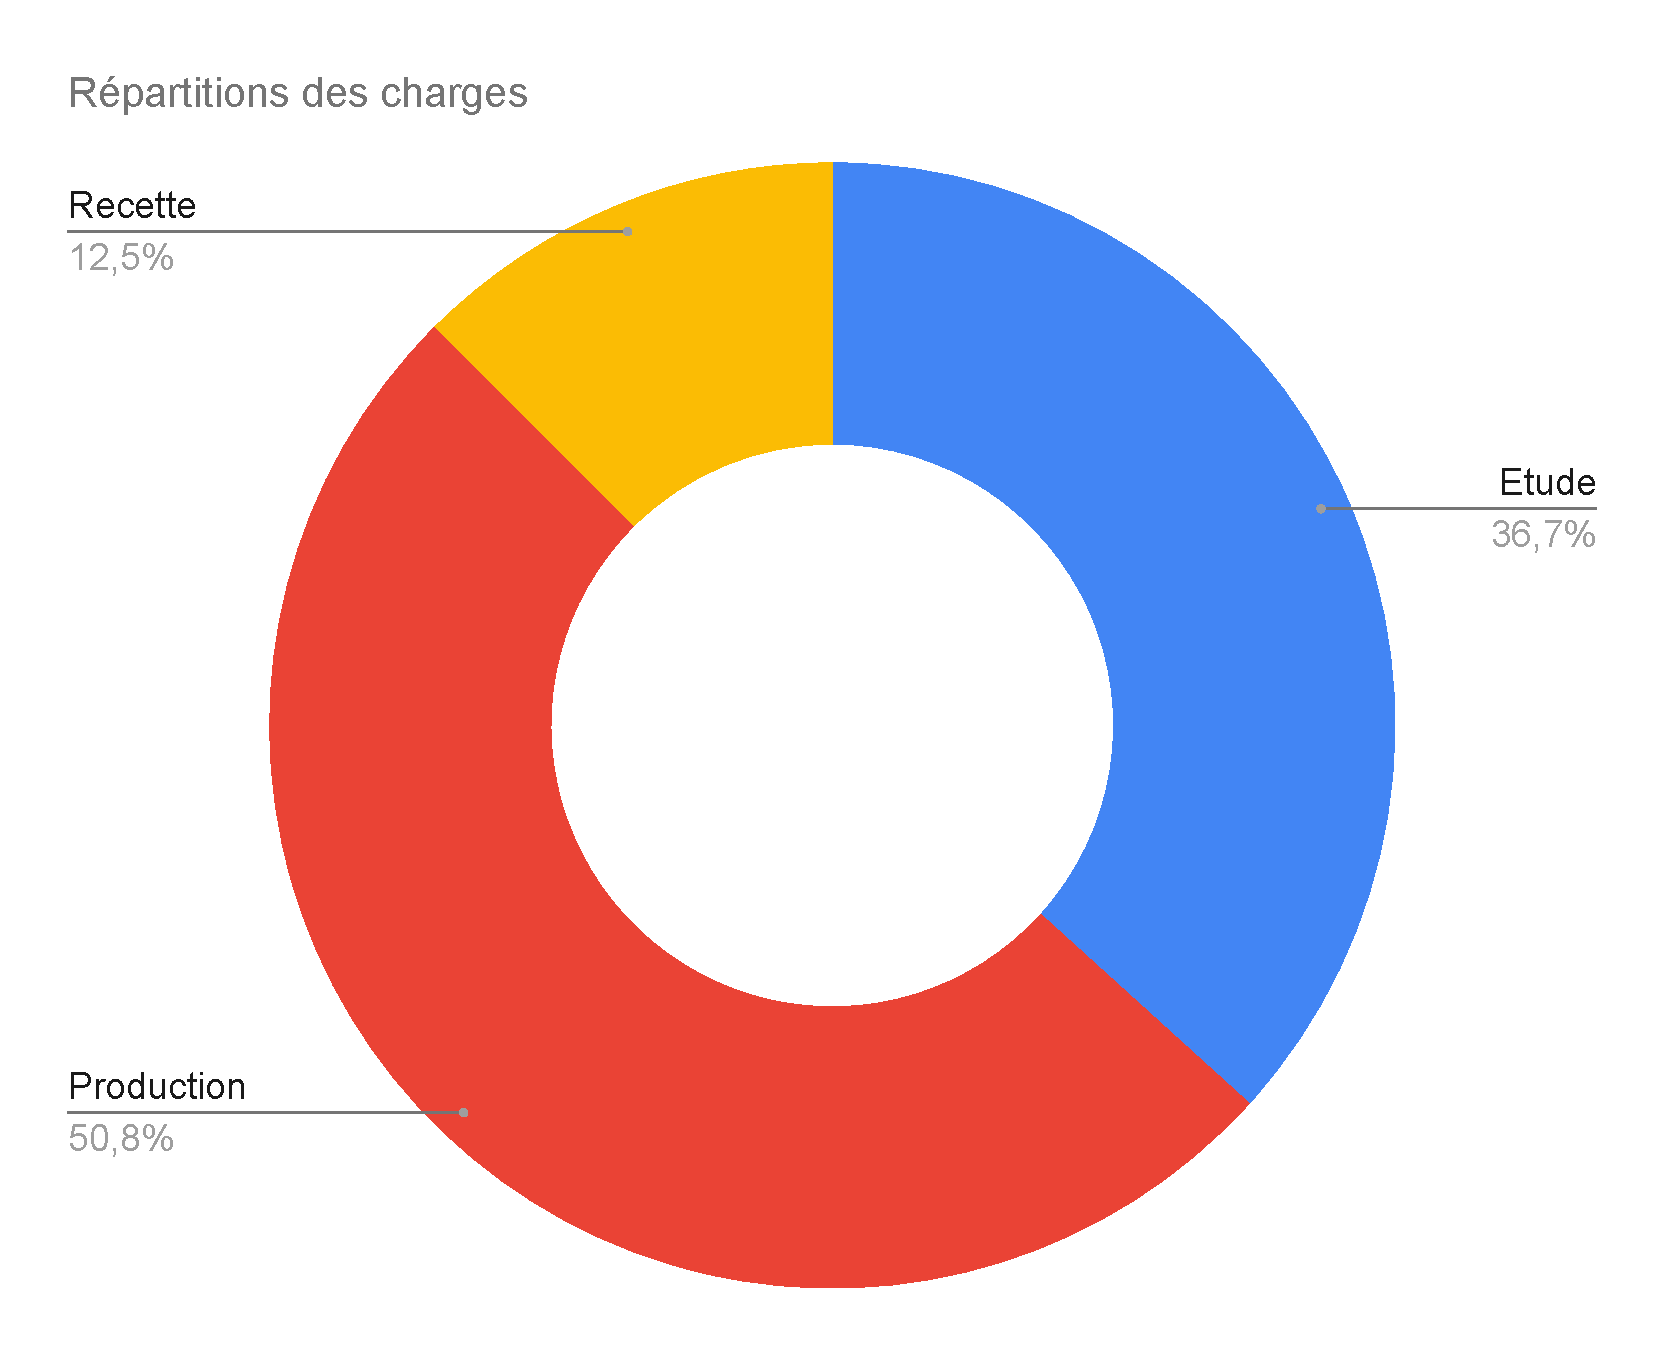
\includegraphics[width=0.8 \textwidth]{Images/repartition_charges.pdf}
    \caption{Graphique de Répartition des charges ramenées en pourcentages.}
\end{figure}

Vous trouverez en figure~\ref{fig:charges_employes} la répartition des charges pour les employés.

\begin{figure}[h]
    \centering
    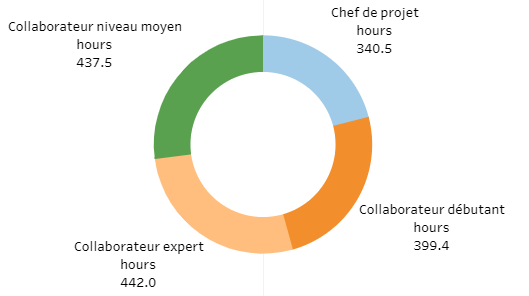
\includegraphics[width=12cm]{Images/charges_employes.png}
    \caption{Répartition du travail par employé}
    \label{fig:charges_employes}
\end{figure}


	\section{Organisation de l'équipe - OBS}
	L'équipe du projet est composée des membres suivants: 
	\begin{itemize}
	    \item Le Chef de projet qui a pour fonction de suivre l'avancement du projet et assurer son bon déroulement.
	    \item L'équipe des développeurs formée de:

	    \begin{itemize}
	        \item Ingénieur Confirmé
	        \item Développeur Mobile
	        \item Développeur junior
	    \end{itemize}
	\end{itemize}
	\begin{figure}[h]
	    \centering
	    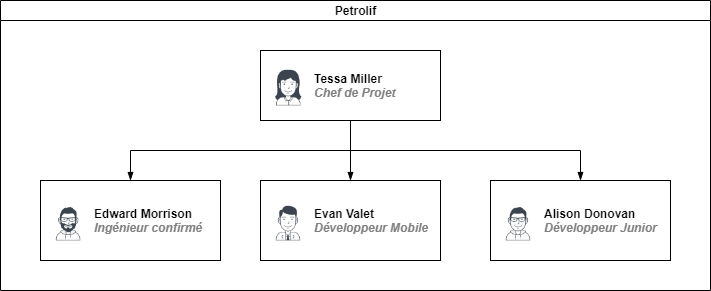
\includegraphics[scale=0.5]{Images/org.png}
	    \caption{Organisation de L'équipe}
	    \label{fig:org}
	\end{figure}
	
	\newpage
	\section{Analyse des risques}

Le projet présente de multiples risques tout au long de ses cycles de développement. Ces évènements auraient pour conséquences de ralentir la progression du projet. Dans le cas où un de ces évènements viendrait à se réaliser, il faudra compter sur une augmentation du coût du projet pour le client et un retard quant à la livraison du produit. Ci dessous, une liste des principaux risques à prendre en compte pour la réalisation du projet.

\begin{itemize}
\item Perte d’un membre dans l’équipe. Cela aurait un impact sur le fonctionnement de l'équipe elle-même. La perte d'un membre peut avoir plusieurs cause, comme une maladie longue durée ou une rupture de contrat. Notre effectif étant déjà limité, la perte d’un membre causerait un retard important du projet.

\item Maladie des membres d'équipe
\item Problème technique, on peut citer par exemple une coupure électrique ou un arrêt serveur
\item Cyber-attaque (Vol ou destruction de données, ransomware…)
\item Surcharge de l'infrastructure 
\end{itemize}

        \subsection*{Plan d’actions de gestion des risques}

Si un membre de l’équipe décide de quitter le projet, il doit avertir l’entreprise au moins 1 mois avant son départ. Ses contributions au projet restent la propriété de l’entreprise. Par ailleurs, il est demandé aux collaborateurs qui quitteraient le projet de s’assurer de la bonne passation des connaissances avant son départ. 

Dans le cas où un collaborateur souhaiterait effectuer du trvail à distance, les coûts dûs à des problèmes techniques seront à sa charge. 

Il est demandé au client de prévoir une infrastructure pour le backup des données ainsi qu'une architecture de redirection ou de protection temporaire du système en cas de surcharge. Par ailleurs, nous recommendons un audit externe régulier de suivi des failles de sécurité afin de limiter les risques liés aux cyber-attaques.

	\newpage
	
	
	
	
	
	
	\section{Coûts}
Les coûts relatifs au projets se décomposent en différents pôles :
\begin{itemize}
    \item Salaires et charges associées
    \item Coût des licences des logiciels utilisés
    \item Matériel utilisé : Postes de travail, équipements de réseaux, serveurs
    \item Frais généraux : locaux, frais de déplacement, fournitures et petit équipement, assurances
\end{itemize}

\vspace{1em}
De plus, les salaires doivent prendre en compte les charges patronales, nous les comptabilisons donc à hauteur de 42\% du salaire brut. Nous y incluons aussi les frais environnants, cette fois à hauteur de 15\% du salaire brut. \\

% \vspace{1em}
\begin{table}[ht]
    \def\arraystretch{1.5}
    \centerline{
    \begin{tabular}{|p{0.3 \textwidth}|p{0.65 \textwidth}|p{0.15 \textwidth}|} 
        \hline
        \textbf{Poste de dépense} & \multicolumn{1}{|c|}{\textbf{Calcul et durées}} & \multicolumn{1}{c|}{\textbf{Coût en euros}} \\ [1ex]
        \hline
        \hline 
        Les salaires d’après le plan 
        des charges journalières &	(1 + 0.42 + 0.15) * (5000 + 4500 + 3000) = 19625 \euro / mois pour 94,17 J	& \\
        \hline
        chef de projet & (1 + 0.42 + 0.15) * 5000 = 7850 \euro / mois &	27 475,00 \euro \\
        \hline
        Dévelopeur expert &	(1 + 0.42 + 0.15) * 5000 = 7850 \euro / mois + 3 mois & 23 550,00 \euro{} \\
        \hline
        Dévelopeur intermédiaire & (1 + 0.42 + 0.15) * 4500 = 7065 \euro / mois + 3 mois & 21 195,00 \euro \\
        \hline
        Développeur débutant & (1 + 0.42 + 0.15) * 3000 = 4710 \euro / mois + 3 mois & 14 130,00 \euro \\
        \hline
        Extras & formations 4000 \euro, matériel et licences logiciels 10000 \euro, déplacement 500 \euro  & 14 500,00 \euro \\
        \hline
        \textbf{TOTAL} & \textbf{Coûts de base sur la durée prévue} & \textbf{100 850,00 \euro} \\
        \hline
        \textbf{Risques et dépassement de budget} & \textbf{20\% en plus du total} & \textbf{121 020,00 \euro} \\
        \hline
    \end{tabular}}
    \caption{Tableau récapitulatif détaillé du calcul des coûts, avec notamment le détails des calculs relatifs aux salaires et aux charges.}
\end{table}

Ces calculs nous permettent d'affirmer que le coût total du projet s'élève à environ 120 000 \euro{}.
	
	\newpage
	\hypertarget{H}{}
	\section{Modalités de validation et de recette - PAQ}
    	Afin d’assurer au client une qualité optimale des livrables, et notamment des 4 applications à développer, notre équipe s’engage à mettre en place un suivi régulier avec le client ainsi que différentes méthodes d’évaluation et de validation des livrables. Le développement notamment, suivra la méthode SCRUM et nos méthodes de validation s’inscrivent directement dans le processus organisationnel de la production. Ce suivi régulier permettra au client de s’assurer que les solutions applicatives développées répondent à ses besoins réels. 

        \subsection*{Processus de validation client au cours du développement}
    Au cours du déroulement de la phase de production, à l’issue de chaque sprint (fin d’une période de développement selon la méthode SCRUM) le client dispose de la dernière version de ou des applications activement développées ou modifiées. À la date de livraison, le client dispose de trois jours ouvrables afin d’assurer un contrôle des modifications et du fonctionnement global de ou des applications livrées. Toute réserve, observation ou demande explicite de modification de la part du client doivent être formulées dans les délais et transmises par écrit à nos services. L’équipe s’engage à ajouter les modifications éventuelles dans les objectifs du sprint en cours, et de fournir ces modifications dans le livrable de fin de sprint suivant. En cas de non-respect de l’échéance susmentionnée, l’équipe ne pourra être tenue pour responsable de la non prise en compte des exigences demandées dans le sprint engagé. Le client devra donc attendre la fin du sprint et la nouvelle période de contrôle qualité afin de pouvoir à nouveau faire part de ses remarques. 
     

\end{document}